\documentclass[AMA,STIX1COL]{WileyNJD-v2}

\articletype{Article Type}%

\usepackage{setspace}
\usepackage{bbm}


\newcommand{\E}{\mbox{E}}
\newcommand{\RF}{\mbox{RF}}
\newcommand{\Ebar}{\overline{\mbox{E}}}
\newcommand{\RFbar}{\overline{\mbox{RF}}}
\newcommand{\boldtheta}{\boldsymbol{\theta}}
\newcommand{\boldgamma}{\boldsymbol{\gamma}}
\newcommand{\CTSo}{\text{CTS}_0}
\newcommand{\CTSp}{\text{CTS}_{\text{plug}}}

\raggedbottom


\begin{document}

\title{Bayesian Meta-analysis of Observational Contingency Table Data with a Nested Monte Carlo Procedure for Estimating Global Effects}

\author[1]{Thomas A. Gibson*}

\author[1]{Robert E. Weiss}


\authormark{GIBSON, WEISS}


\address[1]{\orgdiv{Department of Biostatistics}, \orgname{University of California, Los Angeles}, \orgaddress{\state{California}, \country{USA}}}


\corres{*Thomas A. Gibson \email{tommy.a.gibson@gmail.com}}

\abstract[Summary]{Observational contingency table data arises when study investigators fix neither row nor column totals. Meta-analysis methods for 2$\times$2 contingency table data often tend to focus on estimating select subsets of statistics that one can calculate from values in a contingency table, and methods that attempt to measure ``global" statistics often use naive estimators that do not take into account heterogeneity parameters for random effects. In this paper we present a novel three-random effect (3RE) model, define an estimand for global statistics that takes into account all appropriate variability, and outline a Monte Carlo-within-Markov chain Monte Carlo procedure for sampling from the posterior distribution of the estimand. In an extensive simulation study we show how the proposed Monte Carlo procedure has superior performance to naive methods, and we apply our method to a dataset of observational studies on patients who present to the emergency department with syncope.}

\keywords{Meta-analysis, diagnostic test, Monte Carlo simulation, syncope}

%\jnlcitation{\cname{%
%\author{Williams K.}, 
%\author{B. Hoskins}, 
%\author{R. Lee}, 
%\author{G. Masato}, and 
%\author{T. Woollings}} (\cyear{2016}), 
%\ctitle{A regime analysis of Atlantic winter jet variability applied to evaluate HadGEM3-GC2}, \cjournal{Q.J.R. Meteorol. Soc.}, \cvol{2017;00:1--6}.}

\maketitle

\footnotetext{\textbf{Abbreviations:} CTS, contingency table statistic; PPV, positive predictive value; NPV, negative predictive value; LR, likelihood ratio; RF, risk factor; RE, random effect, E, event.}

\doublespacing

\section{Introduction} \label{sec:intro}


Data from medical studies can often be tabulated in a 2$\times$2 contingency table. The tables have columns stratified by a dichotomous outcome and rows stratified by a dichotomous covariate. Summary statistics from a 2$\times$2 contingency table include positive/negative predictive value (PPV/NPV), sensitivity and specificity (Sens and Spec), and positive and negative likelihood ratios (LR+ and LR-), among others. We will refer to statistics that can be calculated as functions of some or all of the four values in a 2$\times$2 contingency table as a \textit{contingency table statistic} (CTS). For an individual study's table, this would mean using the counts in each cell to calculate an observed CTS, and for a population it would mean using the underlying multinomial cell probabilities to calculate a population CTS. CTSs describe the relationship between the outcome and the covariate, and calculating most CTSs requires conditioning on either rows or columns. Meta-analysis methods for contingency table data reflect this conditioning, and can generally be segregated into two groups that allow inference for different CTSs. 

Meta-analysis models for randomized controlled trials (RCTs) allow inference for \textit{treatment} CTSs (T-CTSs), and naturally condition on the dichotomous covariate treatment/placebo. T-CTSs include the odds ratio (OR), relative risk (RR), risk difference (RD), and positive/negative predictive values (PPV/NPV). A standard random effects model for T-CTSs is given in Smith et al.\cite{smith1995}, with the log-odds ratio $\log(\mbox{OR})$ as the main inference target. The model of Smith et al.\cite{smith1995} has been extended to network meta-analysis with $K$ treatment groups \cite{lu2004combination, dias2013synthesis, zhang2014network}. Models for diagnostic tests allow inference for \textit{diagnostic} CTSs (D-CTSs) that condition on the presence or absence of an adverse event, denoted by E or $\Ebar$. D-CTSs include sensitivity (Sens), specificity (Spec), ORs, and positive/negative likelihood ratios (LR+/LR-). Ma et al.\cite{ma2016multivariate} reviews meta-analysis models that condition on event status, including the summary receiver operating characteristic (SROC) curve \cite{rutter2001, moses1993, lian2019}, bivariate random effects models \cite{reitsma2005, chu2006, arends2008, chu2012bivariate, guo2017bivariate, hoyer2018meta}, and trivariate random effects models \cite{chu2009, ma2018network, wynants2018trivariate}. Models for T-CTSs and D-CTSs are similar in that they use binomial likelihoods conditioning on rows or columns, respectively. Multiple models \cite{chu2009, rutter2001, ma2018network} aim to estimate \textit{global} statistics, synonymously referred to as ``overall", ``summary", or ``population" statistics that are not study-specific. 

An area of medical literature particularly suited to generating 2$\times$2 data is emergency department (ED) visits for syncope (fainting), where around 5-10\% of older syncope patients experience an adverse event in the 30 days after their initial ED visit \cite{gibson2018}. Many studies provide 2$\times$2 tables of counts for dichotomous \textit{risk factors} (RFs) that are regularly collected during an ED visit for syncope patients, including demographics, comorbidities, symptoms, and test characteristics. The syncope data is unique in that 1) it is \textit{observational}, with neither row totals nor column totals fixed by study investigators, and for which we are interested in both T-CTSs and D-CTSs, and 2) given the large number ($>$ 30) of regularly-measured covariates in the ED for syncope patients, we would like to ``weed out" those covariates that are unrelated to the probability of 30-day adverse events. 

To make inference on T- and D-CTSs together we propose a novel 3 random effect (3RE) Bayesian meta-analysis model as an extension of the model in Smith et al.\cite{smith1995}, with study-level random effects on the average log-odds of an event, the $\log(\mbox{OR})$ of the event, and the log-odds of having the risk factor. Existing 3RE models \cite{chu2009, ma2018network, wynants2018trivariate} model the probability of a positive diagnostic test simultaneously with sensitivity and specificity, but their methods use \textit{plug-in estimators}, plugging in hyperparameters to calculate global statistics, to provide \textit{median} estimates of global T-CTSs and D-CTSs. We instead posit that global \textit{mean} effects are more desirable and define a novel estimand, the \textit{expected value of a given statistic for a new study}, which accounts for all appropriate variability, and we outline a procedure to sample from the posterior distribution of the estimand. We use a fully Bayesian approach which has advantages in interpretation and flexibility, and our parameterization is different in that it builds off of Smith et al.\cite{smith1995} with the log(OR) as the natural parameter. Whether or not a risk factor is related to 30-day adverse events corresponds to a natural scientific question in random effects meta-analysis of whether or not the mean $\log(\mbox{OR})$ for a given risk factor is different from zero \cite{higgins2009}. We introduce a mixture spike-and-slab prior distribution \cite{GM1993, GM1997, KM1998, ishwaran2005} on the mean parameter for the random effects on the $\log(\mbox{OR})$ in the 3RE model, which allows us to calculate the posterior probability that the null hypothesis is true. The mixture prior places point mass on the probability that the mean $\log(\mbox{OR}) = 0$ (the spike), and if not 0, models uncertainty in the mean $\log(\mbox{OR})$ with a continuous prior distribution (the slab). 

We present the 3RE meta-analysis model, a nested Monte Carlo procedure for calculating global CTSs, and a spike-and-slab prior on the global log(OR) in Section \ref{sec:3REmodel}. Section \ref{sec:simulation} presents a simulation to show how well the model identifies true zero and non-zero effects and how accurately and precisely the nested Monte Carlo procedure estimates common CTSs as compared with plug-in estimators. Section \ref{sec:syncope} applies the model to our motivating syncope data. The paper closes with discussion. 

\section{Three RE meta-analysis model} \label{sec:3REmodel}

In the usual meta-analysis, each study $i = 1, \dots, S$ reports a 2$\times$2 table of counts $n_{ijk}$ with rows $j = 0, 1$ defined by the absence or presence of a risk factor (RF), denoted $\RFbar$ and RF, and columns $k = 0, 1$ defined by no adverse event ($\Ebar$) or adverse event (E). Let $n_{i1} = n_{i10} + n_{i11}$ and $n_{i0} = n_{i00} + n_{i01}$ be the number of people with or without the risk factor, respectively,  $N_i = n_{i1} + n_{i0}$ be the total sample size in study $i$, and $\pi_{ij}$ is the probability of an adverse event for a patient in study $i$, group $j$ as illustrated in Table \ref{table:RCT_contingency}. Assuming binomial sampling, the standard Bayesian random effects meta-analysis model is 
\begin{align}
n_{ij1} \vert \pi_{ij} & \sim \mbox{Bin}(n_{ij}, \pi_{ij})  \label{eq:likelihood}\\
\mbox{logit}(\pi_{ij}) & =  \left\{
                  \begin{array}{ll}
                    \beta_{i} - \frac{\delta_i}{2} & \quad j=0 \\ 
                    \beta_{i} + \frac{\delta_i}{2} & \quad j=1,
                  \end{array}
                \right. \label{eq:logit}
\end{align}

\noindent where $\mbox{logit}(a) = \log(a/(1-a))$, $0 < a < 1$, $\beta_i$ is a random intercept term for the log-odds of the event for study $i$ and $\delta_i$ is a random effect for the $\log(\mbox{OR})$ of the event in study $i$. We model $\delta_i$ and $\beta_i$ as normal with unknown mean and variance
\begin{align}
\beta_i \vert \beta_0, \sigma^2_{\beta} & \sim \mbox{N}(\beta_0, \sigma^2_{\beta}), \label{eq:betai} \\
\delta_i \vert \delta_0, \sigma^2_{\delta} & \sim \mbox{N}(\delta_0, \sigma^2_{\delta}), \label{eq:deltai} 
\end{align}
\noindent where population means $\beta_0$ and $\delta_0$ and variances $\sigma^2_{\beta}$ and $\sigma^2_{\delta}$ have priors $p(\beta_0)$, $p(\delta_0)$, $p(\sigma_{\beta})$, and $p(\sigma_{\delta})$ which we discuss in Section \ref{sec:priors}. 

With this model we can make inference on T-CTSs. For observational data where we also want to make inference on D-CTSs, we expand model \eqref{eq:likelihood} - \eqref{eq:deltai} to include a random effect $\psi_i = \mbox{P}(\RF \text{ in study } i)$, the probability of a subject having the risk factor in study $i$. Assuming binomial sampling of $n_{i1}$ from $N_i$ as $\mbox{Bin}(N_i, \psi_i)$, we model $\nu_i = \mbox{logit}(\psi_i)$ as normal with unknown mean and cross-study variance $\sigma^2_{\nu}$ on the logit scale
\begin{align}
n_{i1} \vert \psi_i &\sim \mbox{Bin}(N_i, \psi_i) \label{eq:nij} \\
\nu_i \vert \nu_0, \sigma^2_\nu & \sim \mbox{N}(\nu_0, \sigma^2_\nu), \label{eq:nui}
\end{align}
\noindent where the unknown population parameters $\nu_0$ and $\sigma^2_\nu$ have priors $f(\nu_0)$ and $f(\sigma^2_{\nu})$. 

\subsection{Predictive contingency table statistics} \label{sec:CTSs}

There are study-specific and \textit{global} versions of each CTS. Let $\boldsymbol{Y}$ be the data from all $S$ studies, define $\boldtheta_i = (\beta_i, \delta_i, \nu_i)'$, the parameter vector for the $i^{th}$ study, and let $\boldgamma = (\beta_0, \sigma_{\beta}, \delta_0, \sigma_{\delta},\nu_0, \sigma_{\nu})'$ be the vector of hyperparameters. The unknown study-specific CTS$_i$'s are functions of
\begin{align}
\begin{split}
\pi_{i1} &= \mbox{expit}(\beta_i + \delta_i / 2)  \\
\pi_{i0} &= \mbox{expit}(\beta_i - \delta_i / 2)  \\
\psi_i &= \mbox{expit}(\nu_i), 
\end{split} \label{eq:expit}
\end{align}
where $\mbox{expit}(x) = 1 / (1 + \exp(-x))$. The T-CTSs PPV, NPV, RD, and RR for study $i$ are
\begin{equation}
\begin{alignedat}{2}
\mbox{PPV}_i &= \mbox{P}(\E \vert \RF) = \pi_{i1}   \qquad &\mbox{NPV}_i &= \mbox{P}(\Ebar \vert \RFbar) = 1 - \pi_{i0} \label{eq:rowCTS} \\
\mbox{RR}_i &= \frac{\mbox{P}(\E \vert \RF)}{\mbox{P}(\E \vert \RFbar)} = \frac{\pi_{i1}}{\pi_{i0}}  \qquad &\mbox{RD}_i &= \mbox{P}(\E \vert \RF) - \mbox{P}(\E \vert \RFbar) = \pi_{i1} - \pi_{i0} , 
\end{alignedat}
\end{equation}
\noindent and the D-CTSs Sens, Spec, LR$+$, and LR$-$ are
\begin{equation}
\begin{alignedat}{2}
\mbox{Sens}_i &= \mbox{P}(\RF \vert \E) = \frac{\pi_{i1} \psi_i}{\pi_{i1}\psi_i + \pi_{i0}(1 - \psi_i)} \qquad &  \mbox{LR}-_i &= \frac{1 - \mbox{Sens}_i}{\mbox{Spec}_i}  \label{eq:columnCTS} \\
\mbox{Spec}_i &= \mbox{P}(\RFbar \vert \Ebar) = \frac{(1 - \pi_{i0})(1 - \psi_i)}{(1 - \pi_{i0}) (1 - \psi_i) + (1 - \pi_{i1}) \psi_i} \qquad & \mbox{LR}+_i &= \frac{\mbox{Sens}_i}{1 - \mbox{Spec}_i}.
\end{alignedat}
\end{equation}
\noindent Each CTS$_i$ is then a function $g(\boldtheta_i)$ of the study-specific parameters $\boldtheta_i$ for appropriate choice of $g(\cdot)$. 

Usually the purpose of meta-analysis is to consolidate information from multiple studies, and we are interested in \textit{global} rather than study-specific CTSs. Existing methods use \textit{plug-in estimators}, $\text{CTS}_{\text{plug}}(\beta_0, \delta_0, \nu_0)$ as estimates of global CTSs, by plugging in 
\begin{align}
\pi_{1} &= \mbox{expit}(\beta_0 + \delta_0 / 2) \nonumber \\
\pi_{0} &= \mbox{expit}(\beta_0 - \delta_0 / 2). \nonumber \\
\psi &= \mbox{expit}(\nu_0), \nonumber
\end{align}
in equations \eqref{eq:rowCTS} - \eqref{eq:columnCTS} in place of study-specific $\pi_{i1}$, $\pi_{i0}$, and $\psi_i$. The plug-in method ignores 1) the nonlinear relationship between the mean hyperparameters $(\beta_0, \delta_0, \nu_0)$ and the global CTSs, and 2) the heterogeneity present across studies represented by $\sigma_{\beta}$, $\sigma_{\delta}$ and $\sigma_{\nu}$. In contrast, we define the target estimand as the \textit{predictive mean} $\CTSo(\boldgamma)$ \textit{of a CTS for a new study} given $\boldgamma$, $\CTSo(\boldgamma) = \E[g(\boldtheta_{S + 1})\vert \boldgamma]$, where $\boldtheta_{S + 1} = (\beta_{S + 1}, \delta_{S + 1}, \nu_{S + 1})$ and $\beta_{S + 1}, \delta_{S + 1},$ and $\nu_{S + 1}$ are distributed as in \eqref{eq:betai}, \eqref{eq:deltai}, and \eqref{eq:nui}, and study index $i$ can take on value $S + 1$. For brevity, we use $\CTSo \equiv \CTSo(\boldgamma)$ and $\CTSp \equiv \CTSp(\beta_0, \delta_0, \nu_0)$ for the rest of this paper. 

For given $\boldgamma$, we approximate $\CTSo = \E[g(\boldtheta_{S + 1}) \vert \boldgamma]$ with a Monte Carlo estimate 
\begin{equation}
\begin{split}
\E[g(\boldtheta_{S + 1}) \vert \boldgamma] & = \boldsymbol{\int}g(\boldtheta_{S + 1})  P(\boldtheta_{S + 1} \vert \boldgamma)  d\boldtheta_{S + 1} \\
 &\approx \frac{1}{L} \sum_{l=1}^L g(\boldtheta_{S + 1}^{(l)})
\end{split}
\end{equation}
\noindent where $L$ is a pre-specified integer chosen so that Monte Carlo error is desirably small, and $\boldtheta_{S + 1}^{(l)}$ are drawn from the predictive distribution $P(\boldtheta_{S + 1} \vert \boldgamma)$. To draw samples $m = 1, \dots, M$ from the posterior distribution $P(\CTSo \vert \boldsymbol{Y})$ within a Markov chain Monte Carlo (MCMC) algorithm we approximate the integral $\boldsymbol{\int}g(\boldtheta_{S + 1})  P(\boldtheta_{S + 1} \vert \boldgamma) d\boldtheta_{S + 1}$ in each iteration $m$ with a Monte Carlo calculation. Given $M$ MCMC samples $\boldgamma^{(m)}$, $m = 1, \dots, M$ from the posterior of $P(\boldgamma \vert \boldsymbol{Y})$, for each $m$ we
\begin{enumerate} \label{proc:nestedMC}
\item Take $L$ draws $\boldtheta_{S + 1}^{(m, l)}$, $l = 1, \dots, L$ from the predictive distribution $P(\boldtheta_{S + 1}\vert \boldgamma^{(m)})$ and calculate the CTS $g(\boldtheta_{S + 1}^{(m, l)})$ for each of the $L$ draws, 
\item Estimate $\CTSo(\boldgamma^{(m)}) = \E[g(\boldtheta_{S + 1})\vert \boldgamma^{(m)}] \approx \frac{1}{L} \sum_{l=1}^L g(\boldtheta_{S + 1}^{(m, l)})$.
\end{enumerate}
Sampling $\boldgamma^{(m)}$ and $\CTSo(\boldgamma^{(m)})$ in each iteration of MCMC sampling yields approximate samples from the posterior distribution for the expectation of the CTS given data $\boldsymbol{Y}$ and $\boldgamma$, $p(\CTSo \vert \boldsymbol{Y})$, where uncertainty in $\CTSo$ is due to uncertainty in the parameters $\boldgamma$. We refer to this method as the MC procedure.

\subsection{Spike-and-slab prior for the log-odds ratio} \label{sec:spike}

We want to formally test the null hypothesis $H_0{:\,} \delta_0 = 0$ that the $\log(\mbox{OR})$ is 0 against $H_A{:\,} \delta_0 \ne 0$. The Bayesian approach to testing builds an encompassing model where both $H_0$ and $H_A$ have positive probability, for example, with a spike-and-slab (SAS) prior $p_1(\delta_0)$ for $\delta_0$
\begin{align}
\delta_0 & = \left\{
		\begin{array}{ll}
			\delta &\quad \rho = 1 \\
			0 &\quad \rho = 0
		\end{array}
		\right. \label{eq:delta0spike}\\
\rho &\sim \mbox{Bernoulli}(p) \label{eq:spike} \\
\delta &\sim \mbox{N}(0, b_\delta^2), \label{eq:delta}
\end{align}
\noindent where $p$ is the prior probability that $\delta_0 = 0$. In the absence of other prior information we usually choose $p = 0.5$. We call the 3RE model \eqref{eq:likelihood} - \eqref{eq:nui} with prior \eqref{eq:delta0spike} - \eqref{eq:delta} the 3RE-SAS model. In the absence of prior information one can set prior standard deviation $b_\delta = 2$ to give support to values of $\delta_0 \in (-4, 4)$, where a log(OR) $\delta$ of $-4$ or 4 corresponds to an OR of 0.02 or 55. A special case has $\rho = 1$, and $\delta_0 \equiv \delta$, which is a continuous prior for $\delta_0$.

\subsection{Prior distributions for other parameters} \label{sec:priors}

For the mean parameters $\beta_0$ and $\nu_0$ we propose normal distributions with known means $a_{\beta}$, $a_{\nu}$ and variances $b_{\beta}^2$, $b_{\nu}^2$
\begin{align}
\beta_0 &\sim \mbox{N}(a_\beta, b_\beta^2) \label{eq:beta0} \\
\nu_0 &\sim \mbox{N}(a_\nu, b_\nu^2). \label{eq:nu0}
\end{align}
\noindent Prior means $a_\beta$ and $a_\nu$ are prior guesses at the mean log-odds of an event and log-odds of the risk factor, respectively, and the standard deviations $b_\beta$ and $b_\nu$ are chosen to be large enough to give support to all plausible values of the parameters. As a default we assign each of the prior standard deviations $\sigma_\beta$, $\sigma_\delta$, and $\sigma_\nu$ weakly informative half-Cauchy prior distributions
\begin{align}
\sigma_\beta &\sim \mbox{half-Cauchy}(A_\beta) \label{eq:sigmabeta} \\
\sigma_\delta &\sim \mbox{half-Cauchy}(A_\delta) \label{eq:sigmadelta} \\
\sigma_\nu &\sim \mbox{half-Cauchy}(A_\nu) \label{eq:sigmanu}
\end{align}
where $\sigma \sim \mbox{half-Cauchy}(A)$ with scale parameter $A > 0$ has density $p(\sigma) \propto (A^2 + \sigma^2)^{-1} \mathbbm{1}_{[\sigma > 0]}$ \cite{gelman2006prior}. The scale parameters $A_\beta$, $A_\delta$, and $A_\nu$ should generally be set between 0.25 and 1. We should expect standard deviations $\sigma_\beta$, $\sigma_\delta$, and $\sigma_\nu$ to be below 1.5, as values above 1.5 may signal problems with model fit/appropriateness or the data because heterogeneity that large is unlikely to occur naturally. Taking $A = 0.25$ yields a prior probability $P(\sigma < 1.5) \approx 0.9$, while $A = 1$ yields $P(\sigma < 1.5) \approx 0.65$. The choice of $A$ matters less with more studies in the meta-analysis. With fewer than 10 studies we recommend $A \in (0.25, 0.5)$. With very few studies (2 or 3), large standard deviations can lead to specificity having posterior mass very close to 1, inducing calculation problems for the statistic $\mbox{LR}+ = \text{Sens} / (1 - \text{Spec})$.

\subsection{Special case: fixed effect for the log-odds ratio}

If we have evidence that the standard deviation $\sigma_{\delta}$ of random effects $\delta_i$ is small, i.e.\ $\sigma_{\delta} \approx 0$, we can instead model a fixed effect for the log(OR) $\delta_0$ where $\delta_1 = \dots = \delta_S = \delta_0$. Modify \eqref{eq:logit} to 
\begin{align}
\mbox{logit}(\pi_{ij}) & =  \left\{
                  \begin{array}{ll}
                    \beta_{i} - \frac{\delta_0}{2} & \quad j=0 \\ 
                    \beta_{i} + \frac{\delta_0}{2} & \quad j=1,
                  \end{array}
                \right. \label{eq:fixed_logit}
\end{align}
where $\delta_0$ has the SAS prior \eqref{eq:delta0spike} - \eqref{eq:delta}. We call this the 2RE-SAS model. The posterior probability $P(\delta_0 = 0 \vert Y)$ is then the probability that $\delta_i = 0$ for every study $i$ in the analysis, as well as for a future study $S + 1$. Because $\delta_{S+1} = 0$ implies $\pi_{[S+1]1} = \pi_{[S+1]0}$, then $\text{RD}_{[S+1]} = 0$, $\text{RR}_{[S+1]} = 1$, $\text{LR}+_{[S+1]} = 1$, and $\text{LR}-_{[S+1]} = 1$, and the posterior probability $P(\delta_0 = 0 \vert Y)$ is also the posterior probability that $\text{RD}_0 = 0$, $\text{RR}_0 = 1$, $\text{LR}+_0 = 1$, and $\text{LR}-_0 = 1$, where 0 and 1 are the null values for the respective CTSs. This is in contrast to the 3RE-SAS model, where $\delta_0 = 0$ does not imply that RR, RD, LR$+$ and LR$-$ are exactly equal to their null values, as $\sigma_{\delta} > 0$.

\section{Simulation studies} \label{sec:simulation}

We perform three simulations to 
\begin{enumerate}
\item{Determine appropriate choices for $L$ in calculating $\CTSo$ in the MC procedure,}
\item{Compare the MC procedure $\CTSo$ to the plug-in estimator $\CTSp$ with known target values $\CTSo$,}
\item{Assess the posterior probability of the null hypothesis $\delta_0 = 0$ in the 3RE-SAS model.}
\end{enumerate}

\noindent We keep certain conditions equivalent across the three simulations. In all simulations we fix $\beta_0 = \nu_0 = \log(.15 / .85)$ and independently draw the number of subjects for each study from a discrete uniform distribution $\text{Uniform}(250, 2500)$ to match values typical of the syncope data analysis. In each analysis we set 4000 MCMC iterations in each of 4 chains, discard the first 2000 iterations as burn-in and use a thin of 2, leaving 4000 MCMC samples from each posterior. We use prior means $a_{\beta} = a_{\nu} = -1$, prior variances $b_{\beta} = b_{\delta} = b_{\nu} = 4$, and $A_{\beta} = A_{\delta} = A_{\nu} = \frac{1}{\sqrt{2}} \approx .707$. For the SAS prior we use a prior probability $P(\delta_0 = 0) = 0.5$. In each analysis, initial values for mean parameters are drawn independently from a Uniform(-1, 1) distribution, and initial values for random effect standard deviations $\sigma_{\beta}$, $\sigma_{\delta}$, and $\sigma_{\nu}$ are drawn independently from a Uniform(0.2, 1) distribution.

Each simulation varies different factors, and we refer to each combination of factors as a scenario.

\subsection{Simulation 1: Choice of $L$ for Monte Carlo procedure} \label{sec:L}

Simulation 1 consists of two smaller simulations. First we compare posterior standard deviations (SDs) and 95\% interval lengths for LR$+_0$ for several choices of $L$. First, we generate $K_{11} = 100$ datasets for two scenarios -- one with $(\sigma_{\beta}, \sigma_{\delta}, \sigma_{\nu}) = (0.5, 0.5, 0.5)$ and one with $(\sigma_{\beta}, \sigma_{\delta}, \sigma_{\nu}) = (1, 1, 1)$, and we fix $\delta_0 = 2$. Each dataset has $S = 10$ studies. Table \ref{table:L} shows average posterior standard deviations (SDs) and 95\% interval lengths of $\mbox{LR}+_{0}$ for $L \in \{1, 10, 100, 1000, 10000\}$ for the two simulation scenarios. As $L$ increases, estimation variance of $\CTSo(\boldgamma)$ decreases for each $\boldgamma$, and for sufficiently large $L$ the estimation variance is negligible in comparison to the posterior variance. This will be reflected in posterior variance of $\CTSo$ and the posterior interval width for $\CTSo$ decreasing to asymptotes.

Posterior SDs and 95\% credible interval (CI) lengths decrease with increasing $L$, and the effect of further increasing $L$ has a decreasing impact upon SD and 95\% CI length. If true random effect standard deviations $\sigma_{\beta}$, $\sigma_{\delta}$, and $\sigma_{\nu}$ are moderate $(\approx 0.5)$, then $L=100$ is often sufficient. However, if the standard deviations $\sigma_{\beta}$, $\sigma_{\delta}$, and $\sigma_{\nu}$ are large then $L = 1000$ may be preferable and could have an impact on inferences. Taking $L = 10000$ becomes computationally burdensome, and offers little additional precision

In a second simulation, we take two fixed values of $\boldgamma$, $\boldgamma = (\log(\frac{.15}{.85}), 0.5, 2, 0.5, \log(\frac{.15}{.85}), 0.5)$ or $\boldgamma = (\log(\frac{.15}{.85}), 1, 2, 1, \log(\frac{.15}{.85}), 1)$ and calculate  $K_{12} = 2000$ replicates of $\text{LR}+_0$ to estimate the \textit{within-MC} standard deviation $\text{SD}_{\text{within}}$ for $\text{LR}+_0$. Results are shown in Table \ref{table:L-one-gamma}. The bottom row of Table \ref{table:L} with $L = 10000$ offers a close approximation to the \textit{between-MC} standard deviation $\text{SD}_{\text{between}}$ for $\CTSo$. The user's choice of $L$ should depend on the ratio of within-MC SD to between-MC SDs. We recommend at least $\text{SD}_{\text{within}} / \text{SD}_{\text{between}} < 0.1$.. For Simulations 2 and 3 we use $L = 1000$. 


\subsection{Simulation 2: estimating $\CTSo$} \label{sec:sim_CTS}

Simulation 2 evaluates how accurately the posterior mean of $\CTSo$, $\text{E}[\CTSo \vert Y]$, from the 3RE model estimates the true CTS values LR$+_0$, LR$-_0$, $\text{PPV}_0$, $\text{NPV}_0$, $\text{Sens}_0$, and $\text{Spec}_0$ for a new study and how far off the naive plug-in estimator $\CTSp$ is from $\CTSo$. We fix $\delta_0 = 2$, vary $\sigma_{\delta} \in \{0.1, 0.25, 0.5\}$, and vary the number $S$ of studies per meta analysis with $S \in \{10, 30, 50\}$ in a 3$\times$3 factorial design for 9 scenarios. 

Let $T_k$ be the posterior mean of the estimand of interest in simulation iteration $k$, $k = 1, \dots, K$, and define the simulation mean $\overline{T} = \frac{1}{K}\sum_{k=1}^K T_k$ and variance $V_T = \frac{1}{K - 1}\sum_{k=1}^K (T_k - \overline{T})^2$, and let $\mu$ be the known target value that $T_k$ is estimating. We choose $K$ to make the Monte Carlo standard error (MCSE) of relative bias, $\mbox{MCSE(rBias)} = \sqrt{V_T / (K\mu^2)}$, sufficiently small for each scenario. In this simulation we define $T_k$ as the posterior mean $T_k = \E[\CTSo \vert Y_k]$ for the CTSs LR$+$, LR$-$, NPV, PPV, Sens, and Spec. We calculate target values $\mu$ for each scenario by generating 100,000 probability tables from \eqref{eq:logit} - \eqref{eq:expit} using the known hyperparameters $\boldgamma$, calculating the desired CTSs for each probability table, and averaging each CTS across tables. Using a preliminary set of 100 simulations, we calculate $K_2 = 2500$ such that MCSE(rBias) $< 0.0025$ for all scenarios and CTSs. 

We record the posterior mean, SD, and 95\% CI for every CTS for both $\CTSo$ and $\CTSp$ and calculate bias, 95\% CI coverage, average 95\% CI length, and root mean-squared error (RMSE) for the CTSs LR$+$, LR$-$, NPV, PPV, Sens, and Spec. 

Figure \ref{fig:cts_bias} shows bar plots of bias for each CTS, combination of $S$ and $\sigma_{\delta}$, and $\CTSo$ or $\CTSp$. Dotted bars plot the bias for $\CTSp$ and solid bars plot the bias for $\CTSo$. For sample sizes $S = 30$ and 50, $\CTSp$ has bias that is both significantly different from zero and larger than bias for $\CTSo$, with $\CTSp$ bias surprisingly increasing as sample size increases for NPV and Spec, which we comment on in Section \ref{sec:discussion}. There is a similar pattern in Figure \ref{fig:cts_rmse} for RMSE, where RMSE for $\CTSo$ is smaller than for $\CTSp$ when $S \in \{30, 50\}$, although not always significantly. We expect $\CTSo$ to have larger uncertainty than $\CTSp$ because $\CTSo$ accounts for variation in random effects, so an unexpected result in Figure \ref{fig:cts_length} is that the 95\% credible intervals using $\CTSo$ are shorter on average than those of $\CTSp$ for LR$-$ and Sens. The 95\% interval coverage of $\CTSo$ is always greater than or equal to 95\%, while $\CTSp$ coverage falls significantly below 95\% for NPV, PPV, and Spec as $S$ increases for all values of $\sigma_{\delta}$, and for LR$+$ when $\sigma_{\delta}=0.5$. 

Overall, $\CTSo$ from the MC procedure tends to have lower bias and lower RMSE than the plug-in estimator as $S$ increases. It also maintains at least nominal coverage as $S$ increases, while the plug-in estimator sees coverage probabilities fall below nominal levels for multiple CTSs.

\subsection{Simulation 3: true zero and non-zero effects} \label{sec:sim_zero}

For simulation 3, we vary $\delta_0 \in (0, 1, 2)$ and $\sigma_\delta \in (0.1, 0.25, 0.5)$ in a 3$\times$3 factorial experiment with 9 scenarios. The number of simulation iterations $K_3$ is set equal to 1000 so that the posterior probability $T_k = P(\delta_0 = 0 \vert Y_k)$ has MCSE$(\overline{T})< 0.005$. For each scenario we generate $K_3 = 1000$ datasets, where every dataset $Y_k$ has $S = 10$ studies. For each iteration $k = 1, \dots, 1000$ we fit the 3RE-SAS model to data $Y_k$ and calculate $P(\delta_0 = 0 \vert Y_k)$ as the proportion of MCMC samples in which $\rho = 0$. 

Figure \ref{fig:SSP-boxplot} presents boxplots of the distribution of $P(\delta_0 = 0 \vert Y_k)$ for each combination of $(\delta_0, \sigma_\delta)$, and we report the mean and standard deviation of $P(\delta_0 = 0 \vert Y_k)$ for each situation in Table \ref{table:spike-height}. There is a clear distinction in Figure \ref{fig:SSP-boxplot} between simulations with $\delta_0 = 0$ (left-most boxplot in each panel) and simulations with $\delta_0 \ne 0$ (middle and right-most boxplot in each panel). The simulation mean of $P(\delta_0 = 0 \vert Y_k)$ is near zero for true non-zero effects $\delta_0 \in (1, 2)$, and ranges from 0.78 to 0.87 for true mean zero effects $\delta_0 = 0$.

\section{Syncope data analysis: assessing diagnostic utility of regularly measured covariates} \label{sec:syncope}

Syncope, defined as transient loss of consciousness with rapid and spontaneous recovery, accounts for approximately 1.3 million emergency department (ED) visits every year in the United States \cite{probst2015admissions}. Syncope is often harmless, but may be a harbinger of an impending serious cardiac event. ED physicians have difficulty determining which patients are at high risk for an event, and as a result admit up to 85\% of older adults presenting with syncope \cite{birnbaum2008failure} even though only 5-10\% of those presenting to the ED will have an event in the ensuing 30 days \cite{gibson2018}. Given the difficulty of predicting serious cardiac events, we wish to measure the diagnostic value of regularly measured risk factors and determine which risk factors may have zero diagnostic value in predicting 30-day adverse events. Potential risk factors include demographics/comorbidities, symptoms, physical findings, and biomarkers. 

There are 17 studies which each report information on some but not all risk factors; we meta-analyze 31 risk factors for which at least 2 studies provided a 2$\times$2 table. For each analysis we first assess $P(\delta_0 = 0 \vert Y)$ using the 3RE-SAS model and then we re-run the model with continuous prior on $\delta_0$ and summarize posteriors of LR$+_0$, LR$-_0$, $\mbox{PPV}_0$, $\mbox{NPV}_0$, $\mbox{Sens}_0$, and $\mbox{Spec}_0$. If the posterior probability of the risk factor having no effect is $ > 0.5$, one would usually forego computing $\CTSo$ estimates because they would be close to their null values and would be unlikely to provide any diagnostic value. 

Table \ref{table:syncope} details results. Rows are sorted by $P(\delta_0 = 0 \vert Y)$, labeled ``Spike", from lowest to highest. Columns give posterior means and 95\% credible intervals for the CTSs LR$+$, LR$-$, NPV, PPV, Sens, and Spec. Of the 31 risk factors analyzed 20 had posterior probability $\mbox{P}(\delta_0 = 0) \le 0.50$ and 11 had $\mbox{P}(\delta_0 = 0) > 0.50$. Risk factors with more studies have smaller posterior SDs, and risk factors with high posterior probability of specificity near 1 tend to have wider CIs for LR$+_0$. In many circumstances, a threshold of $\mbox{LR}+ > 10$ or $\text{LR}- < 0.1$ are used to either rule in or rule out an impending adverse event with the presence or absence of a risk factor, respectively \cite{deeks2004diagnostic, ranganathan2018understanding}. Here, none of the variables have a posterior mean $\mbox{LR}+_0 > 6.50$ or $\text{LR}-_0 < 0.44$, which highlights the difficulty physicians face in determining which syncope patients are at high risk of an adverse event. 

The biomarkers troponin, urea, and creatinine have the fewest studies in this meta-analysis, but appear to be promising diagnostic predictors of adverse events with large mean values of LR$+_0$. The risk factors age $> 75$, male gender, and abnormal electrocardiogram (ECG) have the highest sensitivities. Figure \ref{fig:syncope_contour} shows contour plots of LR$+_0$ vs LR$-_0$ for the four risk factors with the smallest posterior $P(\delta_0 = 0 \vert Y)$, which are age, male gender, history of congestive heart failure (CHF), and history of heart disease. We see varying degrees of correlation between LR$+$ and LR$-$, with a correlation of $-0.15$ for age and of $-0.94$ for male gender. 

\section{Discussion} \label{sec:discussion}

Given information about a possible future study $S + 1$, such as the probability of the risk factor $\psi_{S+1}$, one can incorporate the information to estimate $\text{CTS}_{[S + 1]}$'s more accurately and precisely. For example, say we know that 5\%, 10\%, or 25\% of people in some new population have elevated blood troponin. Table \ref{table:troponin} lists posterior summaries for $\CTSo$s given known values of P(elevated troponin in new study) $= \psi_{S+1} \in \{.05, .10, .25\}$. We see that rising prevalence of elevated blood troponin corresponds with increasing sensitivity, and decreasing specificity, LR$-$ and LR$+$, while there is no effect on NPV and PPV because NPV and PPV condition on the presence or absence of the risk factor. 

The Monte Carlo-within MCMC procedure to calculate $\CTSo$ is much more quickly implemented with a post-processing procedure rather than being done directly within MCMC. Instead of estimating $\CTSo$ with a Monte Carlo estimate in each iteration of MCMC, extract posterior draws $\boldgamma^{(m)}, m = 1, \dots, M$, and estimate $\CTSo(\boldgamma^{(m)})$ for each $m$ outside of the MCMC algorithm. 

In Section \ref{sec:sim_CTS} we noted that positive bias for $\text{NPV}_{\text{plug}}$ and $\text{Spec}_{\text{plug}}$ increased slightly as the number of studies $S$ per meta-analysis increased. While this is surprising, we believe it is due to to the set of true hyperparameters $\boldgamma$ used to generate data. We used values of $\boldgamma$ which correspond roughly with those seen in the syncope data analysis, which tend to yield values of NPV and Spec close to 1. For a given set of hyperparameters $\boldgamma$, long left tails for the distributions of $\text{NPV}_{\text{new}}$ and $\text{Spec}_{\text{new}}$ are induced through the random effect variation $\sigma_{\beta}$, $\sigma_{\delta}$, and $\sigma_{\nu}$. Larger posterior variance for the mean parameters $\beta_0$, $\delta_0$, and $\nu_0$ can help $\CTSp$ reproduce some of the long left tail in this scenario. However, as $S$ increases and posterior variances of $\beta_0$, $\delta_0$, and $\nu_0$ decrease, less of the skew is captured. 

One can incorporate information from studies that only report a log(OR) $\widehat{\delta}_i$ and its standard error $\text{SE}(\widehat{\delta}_i)$. We say $\widehat{\delta}_i$ was drawn from a normal distribution centered around its true log(OR) $\delta_i$ with variance equal to $\text{SE}(\widehat{\delta}_i)^2$
\begin{align}
\widehat{\delta}_i \vert \delta_i &\sim \mbox{N}(\delta_i, \mbox{SE}(\widehat{\delta}_i)^2), \label{eq:deltahat} 
\end{align}
where the true log(OR) $\delta_i$ is distributed as in \eqref{eq:deltai}. Studies reporting pairs $\big(\widehat{\delta}_i, \mbox{SE}(\delta_i) \big)$ provide information on the mean and variance $(\delta_0, \sigma^2_\delta)$ of the random effects for the log(OR). If there is a set of additional studies reporting 2$\times$2 tables \textit{with fixed row-totals}, we can model them using \eqref{eq:likelihood} - \eqref{eq:betai}. They provide information on $(\delta_0, \sigma^2_\delta)$ and the mean and variance $(\beta_0, \sigma^2_\beta)$ of the random effects for the log-odds of the event but not on the value of $\nu_i$. If the set of additional studies instead have \textit{fixed column-totals}, one can reformulate the model using the ``opposite" parameterization, where the parameters $(\beta_i, \delta_i, \nu_i)$ represent the log-odds of the risk factor, the diagnostic log(OR), and the probability of the event respectively in study $i$. Column totals are often fixed for case-control or diagnostic studies. 

If there is suspected correlation between the random effects $\beta_i$, $\delta_i$, and $\nu_i$, they may be modeled with a multivariate normal distribution
\begin{align}
\begin{pmatrix}
\beta_i \\
\delta_i \\
\nu_i
\end{pmatrix}\sim N\left(\begin{pmatrix}
\beta_0 \\
\delta_0 \\
\nu_0
\end{pmatrix}, \: \boldsymbol{\Sigma} = \begin{pmatrix}
\sigma^2_{\beta} & \rho_{\beta \delta} \sigma_{\beta} \sigma_{\delta}&  \rho_{\beta \nu} \sigma_{\beta} \sigma_{\nu}\\
\rho_{\beta \delta} \sigma_{\beta} \sigma_{\delta} & \sigma^2_{\delta} & \rho_{\delta \nu} \sigma_{\delta} \sigma_{\nu} \\
\rho_{\beta \nu} \sigma_{\beta} \sigma_{\nu} & \rho_{\delta \nu}\sigma_{\delta} \sigma_{\nu} & \sigma^2_{\nu}
\end{pmatrix}\right) \label{eq:mvn_random_effects}
\end{align}
with an inverse-Wishart prior on the covariance matrix. In this paper we model the random effects as independent because the syncope data analysis showed nearly identical results.


There is also potential for meta-analysis results to be used for prior specification in the design and analysis of a future study. The posterior probability $P(\delta_0 = 0 \vert Y)$ can be used to either screen out variables in future analyses, or can be used as prior probabilities in a Bayesian variable selection model using spike-and-slab priors for regression coefficients, as was done in Probst et al.\cite{probst2020faint}.

\bibliography{SpikeSlab}

\clearpage 

%%%%%%%%%%%%%%%
% TABLES
%%%%%%%%%%%%%%%

\begin{table}[!ht]
\centering
\begin{tabular}{c|cc|c}
                           & No Event          & Event       & Total        \\ \hline
j = 0, RF Absent  & $n_{i00} $ & $n_{i01}$    & $n_{i0}$     \\
j = 1, RF Present & $n_{i10}$ & $n_{i11}$    & $n_{i1}$     \\ \hline
j = 0, RF Absent & $1 - \pi_{i0}$    & $\pi_{i0}$  & 1            \\
j = 1, RF Present & $1 - \pi_{i1}$    & $\pi_{i1}$  & 1            \\ \hline 
\end{tabular}
\caption{Sample contingency table for study $i$ with subject counts (top) and a probability representation conditional on presence or absence of the risk factor (bottom).}
\label{table:RCT_contingency}
\end{table}

\clearpage

\begin{table}[!ht]
\centering
\begin{tabular}{lrrrr}
         & \multicolumn{2}{c}{$\sigma_{\beta} = \sigma_{\delta} = \sigma_{\nu} = 0.5$}           & \multicolumn{2}{c}{$\sigma_{\beta} = \sigma_{\delta} = \sigma_{\nu} = 1$}                 \\ 
     \cline{2-5}    $L$ & \multicolumn{1}{r}{SD} & \multicolumn{1}{r}{95\% Length} & \multicolumn{1}{r}{SD} & \multicolumn{1}{r}{95\% Length} \\ \hline
1 & 1.969 & 7.502 & 3.869 & 14.876 \\ 
  10 & 0.868 & 3.360 & 2.295 & 8.646 \\ 
  100 & 0.642 & 2.508 & 1.730 & 6.472 \\ 
  1000 & 0.615 & 2.400 & 1.640 & 6.138 \\ 
  10000 & 0.612 & 2.390 & 1.633 & 6.099 \\ 
\end{tabular}
\caption{Simulation 1: Average posterior standard deviation (SD) and 95\% interval length of $\text{LR}+_{0}$ for different values of $L$ across $K_{11} = 100$ simulation iterations.  \\ 
Second and third columns are results when data was generated with $\sigma_{\beta} = \sigma_{\delta} = \sigma_{\nu} = 0.5$, and in fourth and fifth columns $\sigma_{\beta} = \sigma_{\delta} = \sigma_{\nu} = 1$. \\
SDs and 95\% interval lengths decrease with increasing $L$ with diminishing returns.}
\label{table:L}
\end{table}

\clearpage

\begin{table}[ht]
\centering
\begin{tabular}{lcc}
 & \multicolumn{2}{c}{SD}  \\
  \cline{2-3}
$L$ & $\sigma_{\beta} = \sigma_{\delta} = \sigma_{\nu} = 0.5$ & $\sigma_{\beta} = \sigma_{\delta} = \sigma_{\nu} = 1$ \\ 
  \hline
1 & 1.682 & 4.009 \\ 
  10 & 0.537 & 1.480 \\ 
  100 & 0.173 & 0.500 \\ 
  1000 & 0.054 & 0.155 \\ 
  10000 & 0.017 & 0.051 \\ 
   \hline
\end{tabular}
\caption{Standard deviation across $K_{12} = 2000$ Monte Carlo approximations for LR$+_0$ for two fixed values of $\boldgamma$. We call these values \textit{within-MC} SDs.\\
The mean parameters $\beta_0 = \nu_0 = \log(.15 / .85)$ and $\delta_0 = 2$ are constant across the two scenarios. In the second column, random effect standard deviations are
$\sigma_{\beta} = \sigma_{\delta} = \sigma_{\nu} = 0.5$ and in the third column $\sigma_{\beta} = \sigma_{\delta} = \sigma_{\nu} = 1$.}
\label{table:L-one-gamma}
\end{table}


\clearpage 

\begin{table}[!ht]
\centering
\begin{tabular}{lrrrr}
	&	& \multicolumn{3}{c}{Posterior $P(\delta_0 = 0 \vert Y)$} 
\\ \cline{3-5}
 & $\sigma_\delta$ & $\delta_0 = 0$ & $\delta_0 = 1$ & $\delta_0 = 2$ \\ 
  \toprule
\multirow{3}{*}{Mean} & 0.10 & 0.9113 & 0.0002 & 0.0000 \\ 
  				 & 0.25 & 0.8536 & 0.0023 & 0.0000 \\ 
   				& 0.50 & 0.7917 & 0.0307 & 0.0003 \\ \hline
   \multirow{3}{*}{SD} & 0.10 & 0.0795 & 0.0009 & 0.0000 \\ 
  				 & 0.25 & 0.1156 & 0.0078 & 0.0001 \\ 
  				 & 0.50 & 0.1438 & 0.0582 & 0.0009 \\ 
   \bottomrule
\end{tabular}
\caption{Simulation mean and SD of posterior $P(\delta_0 = 0 \vert Y)$ across 1000 simulation iterations for each combination of $\sigma_{\delta} \in \{0.1, 0.25, 0.5\}$ and $\delta_0 \in \{0, 1, 2\}$.
The first three rows are the mean posterior $P(\delta_0 = 0 \vert Y)$, and the last three rows are the SD of posterior $P(\delta_0 = 0 \vert Y)$.} 
\label{table:spike-height}
\end{table}


\clearpage

\newgeometry{top = 1cm}
\begin{sidewaystable}[h]
\setlength{\tabcolsep}{3.5pt}
\centering
\begin{tabular}{lclllllll}
  \toprule
            &   \multicolumn{1}{c}{Num.}      &	&	   &	     &		&	    &		& \\
 \multicolumn{1}{c}{RF} & \multicolumn{1}{c}{Papers} & \multicolumn{1}{c}{Spike} & \multicolumn{1}{c}{LR+} & \multicolumn{1}{c}{LR-} & \multicolumn{1}{c}{NPV} & \multicolumn{1}{c}{PPV} & \multicolumn{1}{c}{Sens} & \multicolumn{1}{c}{Spec} \\ 
  \toprule
Age &    6 & 0.002 & 2.08 (1.66, 2.65) & 0.44 (0.32, 0.61) & 0.94 (0.85, 0.98) & 0.18 (0.08, 0.34) & 0.71 (0.58, 0.81) & 0.62 (0.51, 0.72) \\ 
  Male Gender &    7 & 0.002 & 1.39 (1.30, 1.50) & 0.72 (0.65, 0.78) & 0.93 (0.83, 0.97) & 0.12 (0.06, 0.25) & 0.58 (0.54, 0.62) & 0.58 (0.57, 0.60) \\ 
  CHF &    8 & 0.004 & 3.43 (2.44, 4.84) & 0.82 (0.74, 0.90) & 0.89 (0.79, 0.95) & 0.26 (0.15, 0.42) & 0.24 (0.16, 0.32) & 0.93 (0.90, 0.95) \\ 
  Heart Disease &    9 & 0.009 & 2.24 (1.69, 2.94) & 0.79 (0.69, 0.88) & 0.92 (0.84, 0.96) & 0.17 (0.10, 0.29) & 0.33 (0.24, 0.44) & 0.84 (0.77, 0.88) \\ 
  Arrhythmia &    6 & 0.010 & 3.09 (2.08, 4.40) & 0.78 (0.63, 0.89) & 0.93 (0.84, 0.97) & 0.18 (0.09, 0.33) & 0.30 (0.17, 0.47) & 0.88 (0.76, 0.94) \\ 
  Dyspnea &    6 & 0.020 & 2.75 (1.88, 4.43) & 0.88 (0.79, 0.94) & 0.87 (0.78, 0.92) & 0.28 (0.18, 0.42) & 0.18 (0.12, 0.28) & 0.93 (0.89, 0.95) \\ 
  Troponin &    3 & 0.056 & 3.90 (1.94, 8.02) & 0.63 (0.38, 0.88) & 0.95 (0.90, 0.97) & 0.21 (0.14, 0.33) & 0.46 (0.22, 0.74) & 0.79 (0.51, 0.93) \\ 
  White Race &    3 & 0.060 & 1.26 (1.10, 1.54) & 0.60 (0.46, 0.80) & 0.94 (0.82, 0.98) & 0.10 (0.04, 0.27) & 0.77 (0.55, 0.89) & 0.36 (0.20, 0.58) \\ 
  ECG &    6 & 0.067 & 2.36 (1.55, 3.68) & 0.60 (0.40, 0.87) & 0.91 (0.82, 0.96) & 0.24 (0.14, 0.38) & 0.57 (0.40, 0.73) & 0.71 (0.58, 0.80) \\ 
  Resp. Rate &    2 & 0.069 & 3.80 (1.80, 8.10) & 0.93 (0.82, 0.98) & 0.90 (0.68, 0.97) & 0.24 (0.09, 0.51) & 0.10 (0.05, 0.22) & 0.97 (0.94, 0.98) \\ 
  Urea &    2 & 0.143 & 6.52 (2.56, 17.09) & 0.82 (0.61, 0.96) & 0.90 (0.68, 0.97) & 0.29 (0.11, 0.56) & 0.21 (0.09, 0.43) & 0.96 (0.90, 0.98) \\ 
  Trauma &    2 & 0.147 & 2.03 (1.22, 3.41) & 0.81 (0.56, 0.97) & 0.93 (0.86, 0.96) & 0.14 (0.08, 0.27) & 0.34 (0.11, 0.69) & 0.77 (0.41, 0.94) \\ 
  Creatinine &    2 & 0.148 & 4.74 (2.05, 12.42) & 0.86 (0.67, 0.96) & 0.90 (0.69, 0.97) & 0.25 (0.09, 0.52) & 0.18 (0.08, 0.38) & 0.95 (0.89, 0.97) \\ 
  CVD &    3 & 0.171 & 1.70 (1.27, 2.38) & 0.92 (0.84, 0.97) & 0.95 (0.82, 0.98) & 0.07 (0.03, 0.24) & 0.17 (0.10, 0.30) & 0.90 (0.80, 0.94) \\ 
  Diabetes &    6 & 0.207 & 1.70 (1.24, 2.29) & 0.88 (0.78, 0.96) & 0.93 (0.83, 0.97) & 0.12 (0.06, 0.24) & 0.26 (0.17, 0.37) & 0.84 (0.77, 0.89) \\ 
  Hematocrit &    7 & 0.211 & 2.56 (1.52, 4.59) & 0.92 (0.82, 0.97) & 0.87 (0.78, 0.93) & 0.23 (0.14, 0.37) & 0.14 (0.07, 0.25) & 0.93 (0.87, 0.96) \\ 
  Hypotension &    5 & 0.232 & 4.92 (1.98, 13.06) & 0.91 (0.78, 0.98) & 0.86 (0.74, 0.93) & 0.32 (0.18, 0.49) & 0.13 (0.06, 0.27) & 0.96 (0.92, 0.98) \\ 
  Pacemaker &    3 & 0.299 & 2.33 (1.21, 4.04) & 0.95 (0.88, 1.00) & 0.87 (0.65, 0.96) & 0.21 (0.07, 0.47) & 0.09 (0.05, 0.16) & 0.96 (0.94, 0.97) \\ 
  Hypertension &    5 & 0.309 & 1.42 (1.08, 1.85) & 0.72 (0.51, 1.00) & 0.93 (0.79, 0.98) & 0.12 (0.05, 0.30) & 0.60 (0.43, 0.75) & 0.55 (0.41, 0.68) \\ 
  Murmur &    4 & 0.311 & 2.29 (1.19, 5.87) & 0.90 (0.72, 1.00) & 0.84 (0.68, 0.92) & 0.26 (0.13, 0.46) & 0.21 (0.08, 0.47) & 0.87 (0.64, 0.96) \\ 
  Oxygen &    2 & 0.508 & 1.69 (1.01, 2.74) & 0.88 (0.69, 1.01) & 0.89 (0.81, 0.93) & 0.17 (0.10, 0.29) & 0.27 (0.13, 0.53) & 0.82 (0.60, 0.91) \\ 
  Seizure &    3 & 0.658 & 1.77 (0.74, 4.64) & 0.97 (0.86, 1.02) & 0.93 (0.75, 0.98) & 0.09 (0.02, 0.29) & 0.08 (0.03, 0.25) & 0.95 (0.84, 0.97) \\ 
  Arr. Rx &    2 & 0.703 & 2.72 (0.55, 11.89) & 0.96 (0.79, 1.06) & 0.81 (0.63, 0.91) & 0.24 (0.09, 0.45) & 0.10 (0.03, 0.29) & 0.94 (0.85, 0.97) \\ 
  Effort &    3 & 0.724 & 1.76 (0.86, 3.73) & 0.95 (0.84, 1.02) & 0.87 (0.76, 0.92) & 0.19 (0.10, 0.33) & 0.12 (0.06, 0.25) & 0.92 (0.86, 0.95) \\ 
  Palpitations &    4 & 0.760 & 1.85 (0.82, 5.22) & 0.96 (0.83, 1.03) & 0.83 (0.69, 0.91) & 0.22 (0.11, 0.41) & 0.12 (0.04, 0.32) & 0.91 (0.75, 0.97) \\ 
  Prev. Syncope &    3 & 0.767 & 0.88 (0.43, 1.82) & 1.07 (0.93, 1.34) & 0.84 (0.68, 0.92) & 0.12 (0.05, 0.29) & 0.15 (0.04, 0.44) & 0.82 (0.53, 0.95) \\ 
  Chest Pain &    3 & 0.785 & 1.65 (0.72, 3.96) & 0.96 (0.85, 1.04) & 0.85 (0.69, 0.93) & 0.18 (0.08, 0.36) & 0.11 (0.05, 0.22) & 0.92 (0.89, 0.94) \\ 
  Stroke &    2 & 0.785 & 1.06 (0.38, 3.11) & 1.06 (0.87, 1.48) & 0.89 (0.75, 0.95) & 0.08 (0.03, 0.22) & 0.16 (0.03, 0.50) & 0.83 (0.48, 0.95) \\ 
  Supine &    2 & 0.786 & 2.06 (0.70, 7.89) & 1.05 (0.56, 2.08) & 0.82 (0.59, 0.93) & 0.23 (0.09, 0.51) & 0.37 (0.11, 0.71) & 0.69 (0.35, 0.91) \\ 
  No Prodromes &    6 & 0.827 & 1.25 (0.85, 1.90) & 0.94 (0.71, 1.27) & 0.90 (0.82, 0.94) & 0.12 (0.07, 0.21) & 0.45 (0.27, 0.64) & 0.60 (0.42, 0.75) \\ 
  Hispanic &    2 & 0.861 & 0.96 (0.50, 1.99) & 1.01 (0.90, 1.09) & 0.89 (0.73, 0.95) & 0.10 (0.04, 0.25) & 0.11 (0.06, 0.24) & 0.88 (0.80, 0.92) \\ 
   \bottomrule
\end{tabular}
\caption{Results of 31 meta-analyses of syncope studies. Each row is for a different risk factor (RF). The second column lists the number of studies that reported a 2$\times$2 table for each RF. Column 3 is the posterior probability $P(\delta_0 = 0 \vert Y)$ from the 3RE-SAS model, sorted from lowest to highest. Columns 4-9 list posterior means and 95\% CIs for LR$+_0$, LR$-_0$, $\text{NPV}_0$, $\text{PPV}_0$, $\text{Sens}_0$, and $\text{Spec}_0$ for each RF. \\
CHF = congestive heart failure; ECG = abnormal electrocardiogram; Resp. Rate = respiratory rate; CVD = cerebrovascular disease; Arr. Rx = arrhythmic medication.} 
\label{table:syncope}
\end{sidewaystable}

\restoregeometry

\clearpage

\newgeometry{margin = 1cm}

\begin{sidewaystable}[ht]
\centering
\begin{tabular}{lllllll}
  \hline
P(RF) & LR- & LR+ & NPV & PPV & Sens & Spec \\ 
  \hline
0.05 & 0.82 (0.67, 0.93) & 5.63 (2.77, 11.25) & 0.95 (0.89, 0.97) & 0.21 (0.13, 0.33) & 0.21 (0.12, 0.36) & 0.96 (0.95, 0.96) \\ 
  0.10 & 0.71 (0.53, 0.88) & 4.47 (2.42, 7.78) & 0.95 (0.89, 0.97) & 0.21 (0.13, 0.33) & 0.35 (0.21, 0.52) & 0.92 (0.90, 0.93) \\ 
  0.25 & 0.53 (0.33, 0.82) & 2.86 (1.80, 4.08) & 0.95 (0.89, 0.97) & 0.21 (0.13, 0.33) & 0.59 (0.39, 0.74) & 0.78 (0.76, 0.81) \\ 
   \hline
\end{tabular}
\caption{Posterior summaries for the RF Troponin given known values of P(RF)$\in \{0.05, 0.10, 0.25\}$ reported as mean (95\% CI).} 
\label{table:troponin}
\end{sidewaystable}

\restoregeometry

%%%%%%%%%%%%%%%%%
%%% FIGURES
%%%%%%%%%%%%%%%%%

\begin{figure}
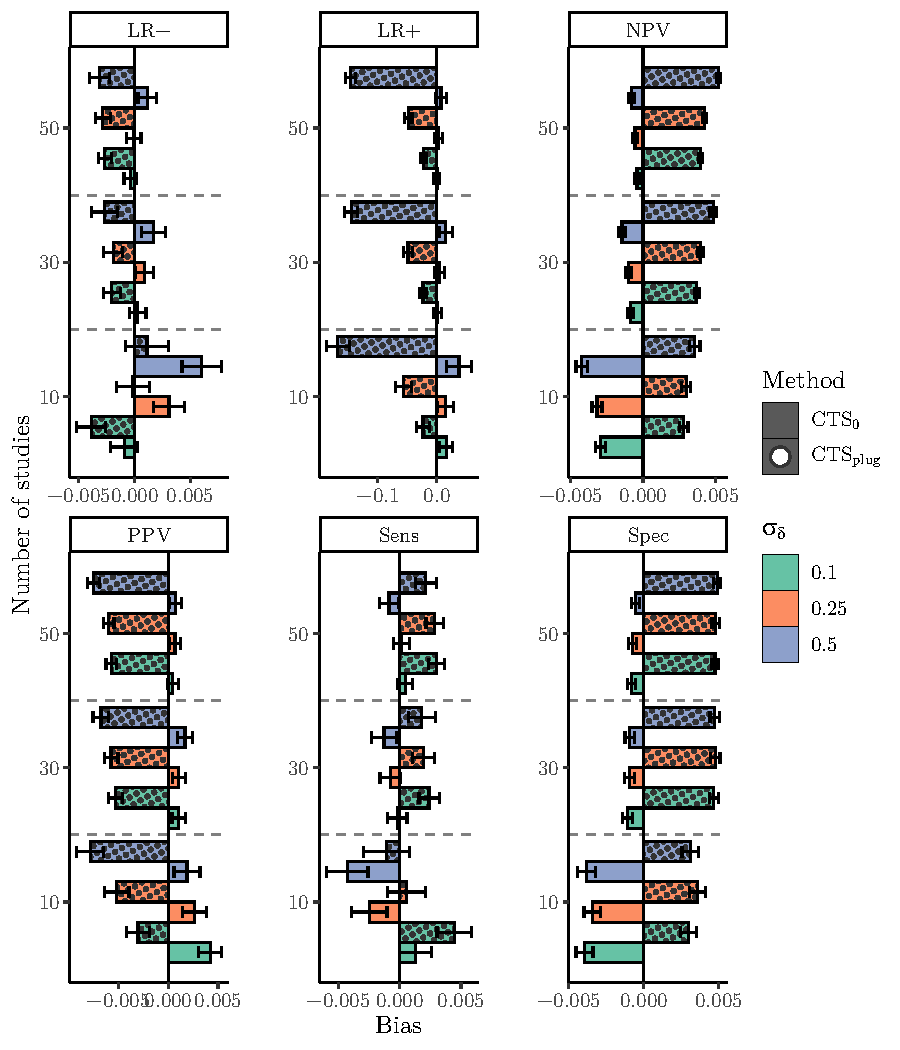
\includegraphics[height = 7in, width = 6in]{bias_plot.pdf}
\caption{Bar plot of bias for each CTS and for each combination of $S \in \{10, 30, 50\}$ on the y-axis and $\sigma_{\delta} \in \{0.1, 0.25, 0.5\}$ indicated by green, red, and blue, respectively. \\
Dotted bars plot bias for the plug-in estimator $\CTSp$ and solid bars plot bias for the Monte Carlo estimator $\CTSo$. Error bars represent $\pm 1.96 \times \text{MCSE}$.}
\label{fig:cts_bias}
\end{figure}

\begin{figure}
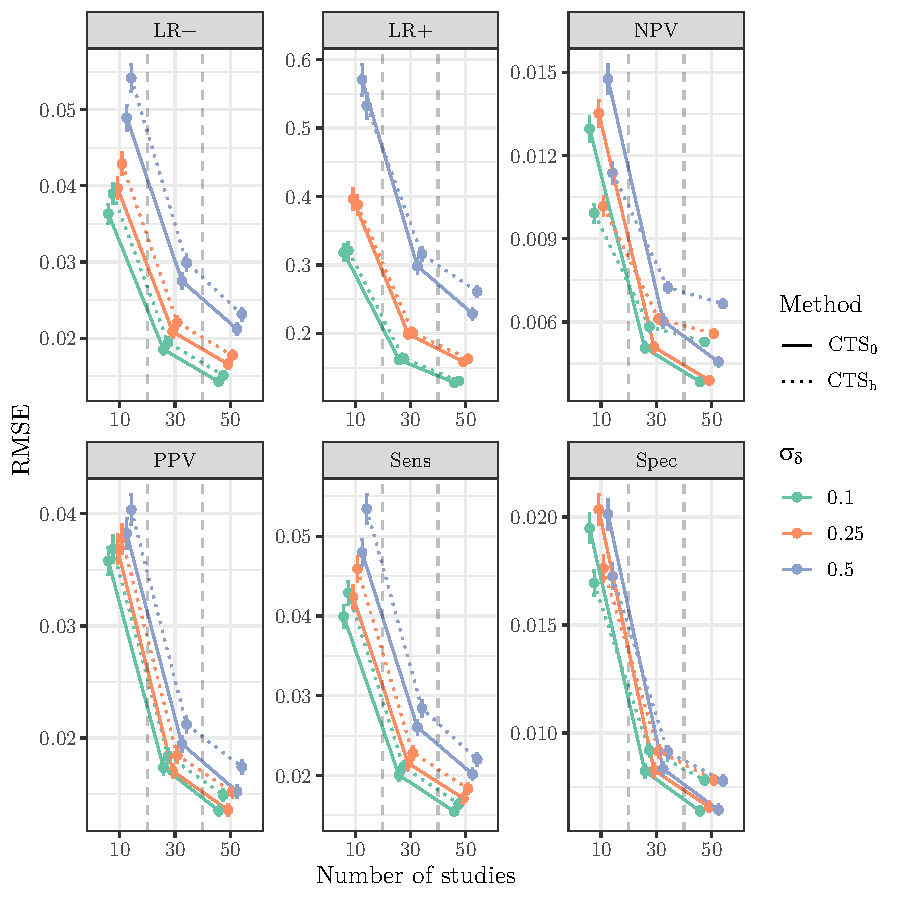
\includegraphics[height = 6in, width = 6in]{rmse_plot.pdf}
\caption{Plot of RMSE for $\CTSo$ (solid lines) and $\CTSp$ (dotted lines). Each panel plots RMSE for a different CTS against sample size $\in \{10, 30, 50\}$ on the x-axis and $\sigma_{\delta} \in \{0.1, 0.25, 0.5\}$ indicated by green, red, and blue lines, respectively. Vertical error bars plot $\pm 1.96 \times \text{MCSE}$.}
\label{fig:cts_rmse}
\end{figure}

\begin{figure}
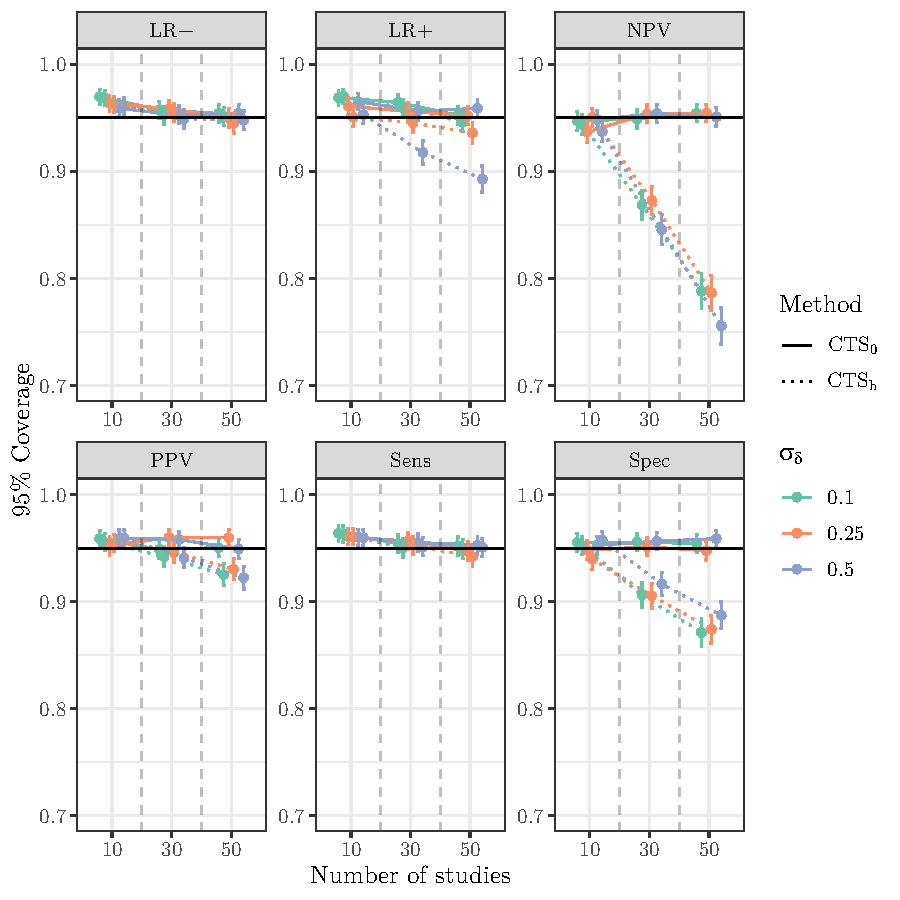
\includegraphics[height = 6in, width = 6in]{cover_plot.pdf}
\caption{Coverage probabilities for 95\% posterior intervals (PIs) for $\CTSo$ (solid lines) and $\CTSp$ (dotted lines) methods. Each panel plots coverage probability for different a different CTS against sample size $\in \{10, 30, 50\}$ on the x-axis, with $\sigma_{\delta} \in \{0.1, 0.25, 0.5\}$ indicated by green, red, and blue lines respectively. Vertical bars plot $\pm 1.96 \times \text{MCSE}$.}
\label{fig:cts_coverage}
\end{figure}

\begin{figure}
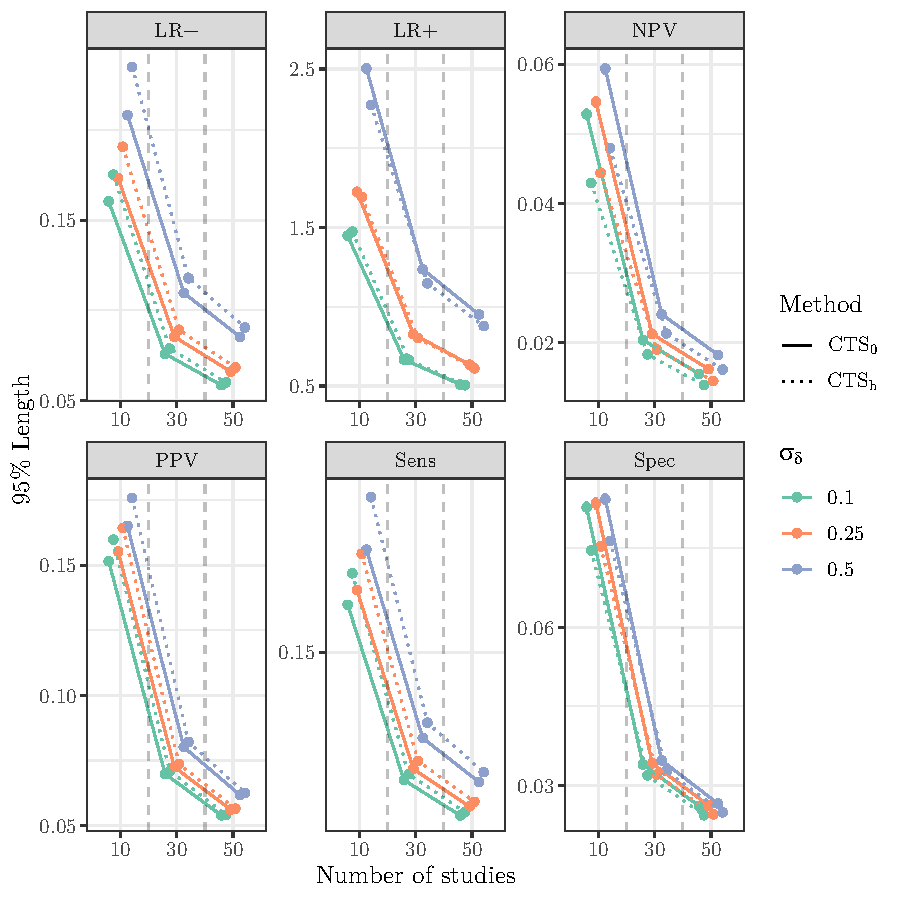
\includegraphics[height = 6in, width = 6in]{length_plot.pdf}
\caption{Average 95\% posterior interval (PI) lengths for $\CTSo$ (solid lines) and $\CTSp$ (dotted lines). PI endpoints were taken as the $2.5^{\text{th}}$ and $97.5^{\text{th}}$ posterior quantiles. Each panel plots average 95\% PI length for a different CTS against sample size $\in \{10, 30, 50\}$ on the x-axis, and $\sigma_{\delta} \in \{0.1, 0.25, 0.5\}$ indicated by green, red, and blue lines respectively. Vertical bars, though difficult to see for most points, plot $\pm 1.96 \times \text{MCSE}$.}
\label{fig:cts_length}
\end{figure}

\begin{figure}
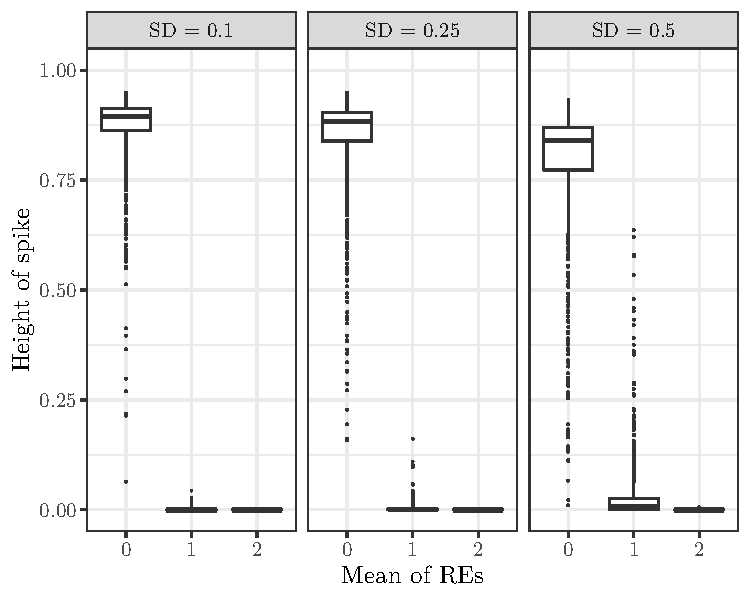
\includegraphics[height = 4in, width = 5in]{spike_boxplot.pdf}
\caption{Boxplots of posterior $P(\delta_0 = 0)$ for each combination of $\sigma_\delta$ and $\delta_0$} in simulation 3. 
\label{fig:SSP-boxplot}
\end{figure}

\begin{figure}
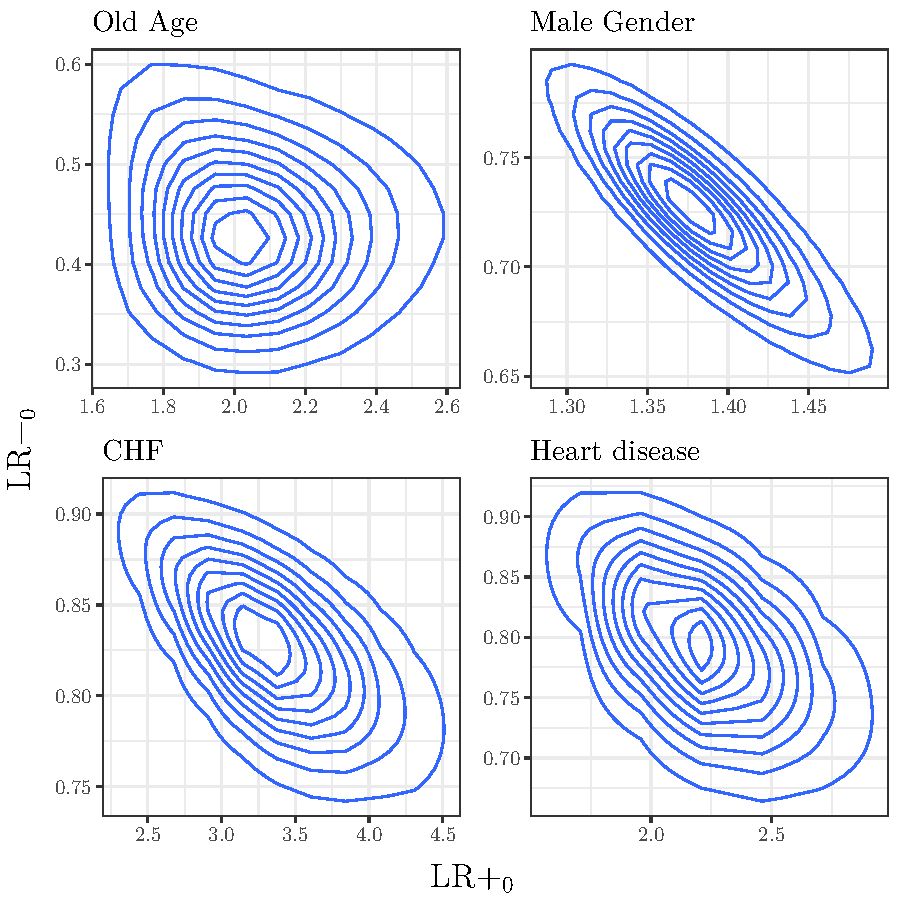
\includegraphics[height = 6in, width = 6in]{syncope_contour.pdf}
\caption{Posterior contour plots of LR$-$ on the y-axis against LR$+$ on the x-axis for the four syncope risk factors with the smallest posterior $P(\delta_0 = 0 \vert Y)$. 
These are old age, male gender, history of congestive heart failure (CHF), and history of heart disease. \\
Higher (lower) values of LR$+$ (LR$-$) signal stronger diagnostic utility.}
\label{fig:syncope_contour}
\end{figure}




\end{document}  